\subsection{Cola}

Una cola es una estructura de datos en la que el modo de acceso a sus elementos es de tipo FIFO
(del inglés \emph{First In First Out}, primero en entrar, primero en salir) que permite almacenar y recuperar
datos.Así, los elementos sólo se pueden eliminar por el principio y sólo se pueden añadir por el final
de la cola.

% TODO: \usepackage{graphicx} required
\begin{figure}[h!]
	\centering
	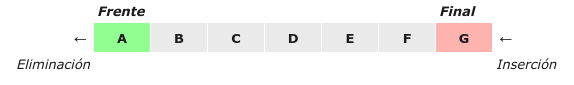
\includegraphics[width=0.7\linewidth]{img/cola}
	\label{fig:cola}
\end{figure}


La estructura independientemente del lenguaje presenta un grupo de funciones para poder manipular los datos que en ella se almacena.

\subsubsection{C++}

Para la utilización de está estructura es necesario añadir en la cabecera del programa \textbf{\#include
<queue>}, gracias a esto ya podemos utilizar la estructura de otro modo no. La clase \textbf{queue} es
genérica.

\begin{itemize}
	\item \textbf{queue::empty():} Devuelve si la cola está vacía.
	\item \textbf{queue::size():} Devuelve el tamaño de la cola.
	\item \textbf{queue::swap():} Intercambia el contenido de dos colas, pero las colas deben ser del mismo tipo, aunque los tamaños pueden diferir.
	\item \textbf{queue::emplace():} Inserta un nuevo elemento en el contenedor de la cola, el nuevo elemento se agrega al final de la cola.
	\item \textbf{queue::front():} Devuelve una referencia al primer elemento de la cola.
	\item \textbf{queue::back():} Devuelve una referencia al último elemento de la cola.
	\item \textbf{queue::push(g):} Agrega el elemento 'g' al final de la cola.
	\item \textbf{queue::pop():} Elimina el primer elemento de la cola.
\end{itemize}

\subsubsection{Java}

Para la utilización de está estructura es necesario importar del paquete java dentro del subpaquete util la clase \emph{Queue} \textbf{import java.util.Queue;} , gracias a esto ya podemos utilizar la estructura de otro modo no.

\begin{itemize}
	\item \textbf{add boolean add(E e):} Agrega el elemento e a la cola al final (cola) de la cola sin violar las restricciones de capacidad. Devuelve verdadero si tiene éxito o IllegalStateException si la capacidad está agotada.
	\item \textbf{peek E peek():} Devuelve la cabeza (frente) de la cola sin eliminarla.
	\item \textbf{element E element():} Realiza la misma operación que el método peek(). Lanza NoSuchElementException cuando la cola está vacía.
	\item \textbf{remove E remove():} Elimina la cabeza de la cola y la devuelve. Lanza NoSuchElementException si la cola está vacía.
	\item \textbf{poll E poll():} Elimina la cabeza de la cola y la devuelve. Si la cola está vacía, devuelve nulo.
	\item \textbf{size int size():} Devuelve el tamaño o el número de elementos en la cola.
	\item \textbf{Offer	boolean offer(E e):} Inserta el nuevo elemento e en la cola sin violar las restricciones de capacidad.
\end{itemize}

\subsection{Pila}

Una pila es una estructura de datos en la que el modo de acceso a sus elementos es de tipo LIFO (del
inglés \emph{Last In First Out}, último en entrar, primero en salir) que permite almacenar y recuperar datos.
Para el manejo de los datos se cuenta con dos operaciones básicas: \textbf{apilar}, que coloca un objeto en
la pila, y su operación inversa, \textbf{des-apilar} (retirar), que retira el último elemento apilado.
La clase \textbf{stack} es genérica.

\begin{figure}[h!]
	\centering
	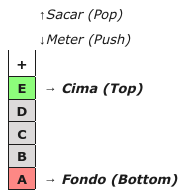
\includegraphics[width=0.20\linewidth]{img/pila}
	\label{fig:pila}
\end{figure}



La estructura independientemente del lenguaje presenta un grupo de funciones para poder manipular los datos que en ella se almacena.

\subsubsection{C++}

Para la utilización de está estructura es necesario añadir en la cabecera del programa \textbf{\#include
	<stack>}, gracias a esto ya podemos utilizar la estructura de otro modo no.

\begin{itemize}
	\item \textbf{stack::top():} Devuelve el elemento que esta en el tope de la pila.
	\item \textbf{stack::empty():} Está función retorna verdad si la pila está vacía y retorna falso si es que por lo menos
	tiene un elemento como tope.
	\item \textbf{stack::size():} Está función retorna cuantos elementos tiene la pila, pero sin embargo no se puede
	acceder a ellas por lo que no es muy usual el uso de está función.
	\item \textbf{stack::push(g):} Agrega el elemento 'g' al tope de la pila.
	\item \textbf{stack::pop():} Elimina el elemento que esta en el tope de la pila.
\end{itemize}

\subsubsection{Java}

Para la utilización de está estructura es necesario importar del paquete java dentro del subpaquete util la clase \emph{Stack} \textbf{import java.util.Stack;} , gracias a esto ya podemos utilizar la estructura de otro modo no.

\begin{itemize}
	\item {\bf push:} Adiciona al tope de la pila el elemento pasado por parámetro 
	
	\item {\bf pop:} Elimina y devuelve el elemento que esta en el tope de la pila siempre que esta tenga elemento, en caso de estar vacia se lanza una excepción.
	
	\item {\bf peek:} Devuelve el elemento sin eleiminarlo que esta en el tope de la pila siempre que esta tenga elemento, en caso de estar vacia se lanza una excepción.

	\item {\bf empty:} Comprueba si la pila esta vacia. Devuelve verdadero si la pila esta vacia y falso en caso contrario.
	
	\item {\bf search:} Busca un elemento de la pila y devuelve la posición con respecto al tope de la pila donde se encuentra la primera ocurrencia del elemento. En caso que el elemento fuera el tope de la pila el valor devuelto sería 1 y así sucesivamente se iría incrementando a medida que se alejara del tope. En caso que elemento no este el valor devuelto será -1.	
\end{itemize}

